\documentclass{howto}
% \usepackage{distutils}
\usepackage{palatino}
\renewcommand{\ttdefault}{cmtt}
\renewcommand{\sfdefault}{cmss}
\newcommand{\myhdl}{\protect \mbox{MyHDL}}
\usepackage{graphicx}
% $Id$

\title{What's New in \myhdl\ 0.3}
\release{0.3}
\author{Jan Decaluwe}
\authoraddress{\email{jan@jandecaluwe.com}}

\begin{document}
\maketitle
\tableofcontents


\section{VCD output for waveform viewing\label{section-wave}}

\ifpdf
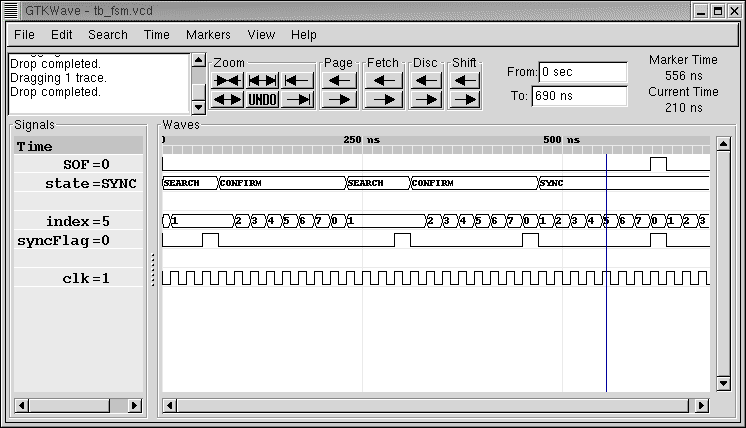
\includegraphics{tbfsm.png}
\fi

\myhdl\ now has support for waveform viewing. During simulation, signal
changes can be written to a VCD output file.  The VCD file can then be
loaded and viewed in a waveform viewer tool.

The user interface of this feature consists of a single function,
\function{trace_sigs()}.  To explain how it works, recall that in
\myhdl{}, instances are created by calling a function that returns a
sequence of generators. For example:

\begin{verbatim}
tb_fsm = testbench()
\end{verbatim}

The \code{tb_fsm} variable is subsequently passed 
as an argument to a \class{Simulation} object constructor
for simulation. To enable VCD tracing, the instance should 
be created as follows instead:

\begin{verbatim}
tb_fsm = trace_sigs(testbench)
\end{verbatim}

As a result, all signals in the hierarchy of the instance will be
traced in an output VCD file called \file{tb_fsm.vcd}. Note that the
argument of \function{trace_sigs()} consists of the uncalled
function. By calling the function under its control,
\function{trace_sigs()} gathers information about the hierarchy and
the signals to be traced.  In addition to a function argument,
\function{trace_sigs()} accepts an arbitrary number of non-keyword and
keyword arguments that will be passed to the function call.

The restrictions on VCD tracing are as follows. First, only
\class{Signal} objects can be traced. Second, only a hierarchy of
instances returned by a pre-simulation top level function call can be
traced. Also, all instances to be traced should have a name: this is
done by assigning the result of an instantiating function call to a
local variable (instead of using it directly.)

Signals are dumped in a suitable format. This format is inferred at
the \class{Signal} construction time, from the type of the initial
value. In particular, \class{bool} signals are dumped as single
bits. (This only works starting with Python2.3, when \class{bool} has
become a separate type).  Likewise, \class{intbv} signals with a
defined bit width are dumped as bit vectors. To support the general
case, other types of signals are dumped as a string representation, as
returned by the standard \function{str()} function.


\end{document}
